% =============================================================================================
%  Slides pour la visio avec O. Le Maître (04/11/2026) : la structure de notre algorithme
%  (vpp_acceleration, run_real_vpp.py), étape par étape avec ses subtilités, et les résultats du
%  8e run. Nos notations seulement.
%  Figures : doc/scripts/fig_profile.py, fig_run8.py (et fig_alc_variance.py pour le chiffre ×5).
%  Compilation : tectonic -X compile slides_le_maitre.tex --outdir build
% =============================================================================================
\documentclass[aspectratio=169,10pt]{beamer}
\usepackage{fontspec}
\usepackage[french]{babel}
\usepackage{amsmath,amssymb,bm,mathtools}
\usepackage{booktabs}
\usepackage{tikz}
\usetikzlibrary{arrows.meta,positioning}

\setbeamertemplate{navigation symbols}{}
\setbeamertemplate{section in toc}[sections numbered]
\setbeamertemplate{footline}[frame number]
\setbeamercolor{frametitle}{fg=blue!40!black}
\setbeamercolor{structure}{fg=blue!40!black}
\setbeamerfont{frametitle}{size=\large,series=\bfseries}

\newcommand{\E}{\mathbb{E}}
\newcommand{\Var}{\mathrm{Var}}
\newcommand{\tp}{^{\mathsf{T}}}
% two-column step slide: what the step does / its subtleties
\newcommand{\quoi}{\textbf{\color{blue!40!black}Ce que fait l'étape}\par\smallskip}
\newcommand{\subtil}{\textbf{\color{orange!70!black}Les subtilités, et pourquoi}\par\smallskip}

\title{Optimisation de la section du C-foil}
\subtitle{Structure de l'algorithme et résultats du 8\textsuperscript{e} run}
\author{Adrian Cozma}
\date{4 novembre 2026}

\begin{document}

\begin{frame}
\titlepage
\end{frame}

% =============================================================================================
\section{Le problème}
% ---------------------------------------------------------------------------------------------
\begin{frame}{Le problème et l'idée}
\begin{columns}[T]
\begin{column}{0.52\textwidth}
\small
\textbf{Le problème}
\[
  \max_{z}\; J(z) = \sum_{c} \omega_c\, V_c(z)
  \quad\text{sous}\quad I_{xx}(z) \ge I_{xx}^{\text{actuelle}}
\]
\begin{itemize}\setlength{\itemsep}{1pt}
  \item $z \in \mathbb R^{10}$ : scores PCA des 16 poids de Kulfan de la section.
  \item $V_c(z)$ : vitesse donnée par la VPP (MDS) à la condition de vent $c$, réglages et équilibre
        optimisés.
  \item $\omega_c$ : poids de la condition dans le profil d'usage (49 conditions).
\end{itemize}

\textbf{La difficulté}
\begin{itemize}\setlength{\itemsep}{1pt}
  \item Une VPP appelle le foil des centaines de fois ; AVL $\times$ XFOIL prend environ 18 s par appel.
  \item Il faut donc un modèle rapide du foil, juste là où la VPP navigue.
\end{itemize}
\end{column}
\begin{column}{0.46\textwidth}
\small
\textbf{L'idée}
\begin{enumerate}\setlength{\itemsep}{2pt}
  \item Un modèle par processus gaussien des efforts du foil, $\hat C(z, a)$, à deux niveaux de fidélité.
  \item La VPP tourne sur la moyenne de ce modèle.
  \item On ne calcule les codes que là où une erreur du modèle change la \textbf{vitesse} : près des
        équilibres de la VPP, pondéré par la sensibilité de la vitesse aux efforts.
  \item On cherche la section en même temps qu'on apprend le modèle.
\end{enumerate}

\medskip
\textbf{Résultat du run 8} : +0,256 nd (+1,9\,\%) sur le profil, en 2 h 30 de boucle ; plan final de 1\,175 points (899 BF, 276 HF).
\end{column}
\end{columns}
\end{frame}

% ---------------------------------------------------------------------------------------------
\begin{frame}{Le profil d'usage : où le bateau navigue vraiment}
\begin{columns}[T]
\begin{column}{0.58\textwidth}
\centering
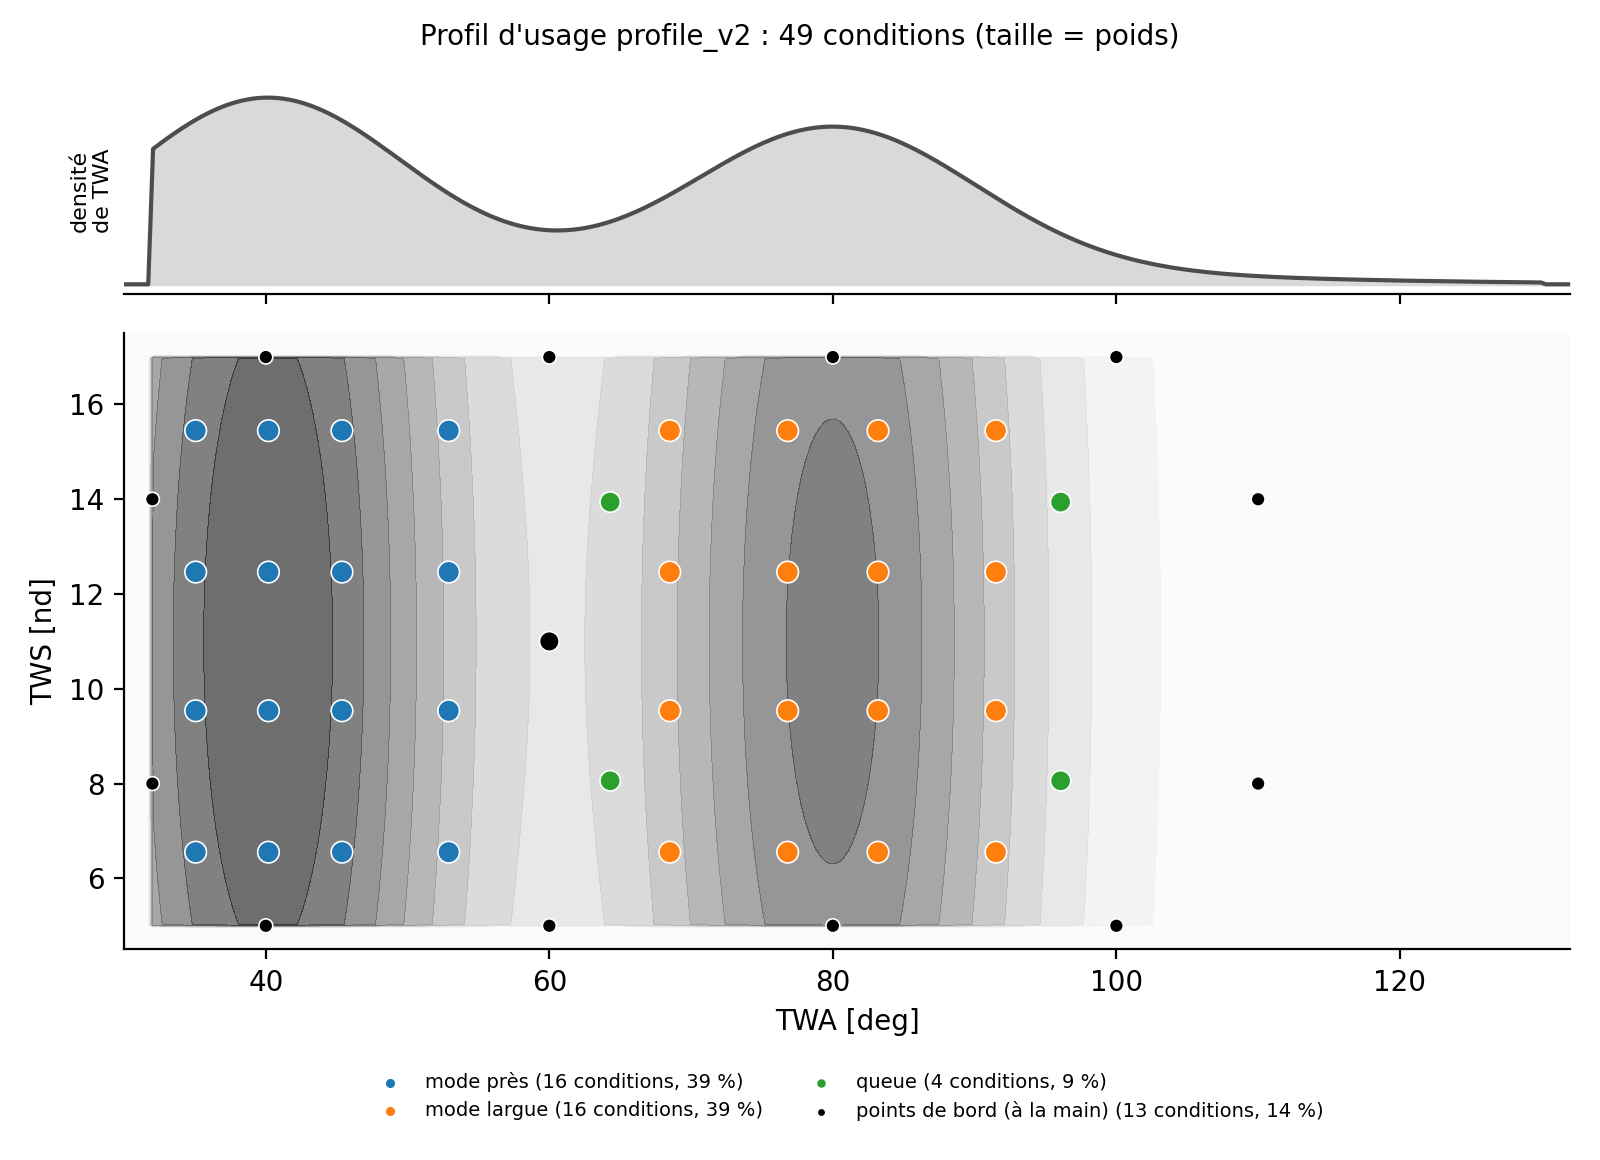
\includegraphics[width=\linewidth]{figures/profile_v2.png}
\end{column}
\begin{column}{0.40\textwidth}
\small
\begin{itemize}\setlength{\itemsep}{3pt}
  \item Deux bosses en TWA : \textbf{près} vers 40° et \textbf{largue} vers 80°, 45\,\% chacune, plus une queue
        du portant (10\,\%).
  \item TWS presque uniforme sur [5, 17] nd. Sous 5 nd, ce n'est pas un cas d'usage ; au-dessus de 17 nd, la
        VPP bute sur sa borne de 24 nd.
  \item \textbf{Points de bord}, posés à la main (14\,\% au total) : la section ne doit pas s'effondrer aux bords
        du domaine.
  \item Les 49 conditions sont celles de la recherche ; leurs poids pèsent l'objectif, le criblage et le choix
        des calculs.
\end{itemize}

\end{column}
\end{columns}
\end{frame}

% =============================================================================================
\section{L'algorithme}
% ---------------------------------------------------------------------------------------------
\begin{frame}{L'algorithme : une boucle}
\centering
\begin{tikzpicture}[node distance=2.6mm, every node/.style={font=\footnotesize, align=left},
  box/.style={draw, rounded corners=2pt, fill=blue!4, text width=12.6cm, inner sep=2.5pt},
  side/.style={draw, rounded corners=2pt, fill=gray!8, text width=12.6cm, inner sep=2.5pt},
  arr/.style={-{Stealth[length=2mm]}, thick}]
\node[side] (init) {\textbf{Départ} : 256 calculs BF et 64 HF répartis dans le domaine ; on ajuste le modèle.};
\node[box, below=of init] (s1) {\textbf{1. Choisir la meilleure section} : on trie 256 sections avec le modèle, puis
  VPP complète des 4 meilleures.\\
  \textcolor{orange!70!black}{\emph{La VPP dépend de son point de départ : on la lance de plusieurs départs et on
  garde le plus rapide.}}};
\node[box, below=of s1] (s2) {\textbf{2. Mesurer la sensibilité de la vitesse aux efforts} : on décale chaque
  effort du modèle et on refait la VPP.\\
  \textcolor{orange!70!black}{\emph{Une erreur sur la traînée compte bien plus qu'une erreur sur les autres
  efforts.}}};
\node[box, below=of s2] (s3) {\textbf{3. Choisir 16 calculs} : ceux qui réduisent le plus l'incertitude sur la
  \emph{vitesse}, par unité de coût, près des équilibres de la VPP ; le critère choisit aussi le code (BF ou HF).\\
  \textcolor{orange!70!black}{\emph{L'incertitude du modèle ne dépend que de la position des points, pas des
  résultats : on peut en choisir 16 d'un coup.}}};
\node[box, below=of s3] (s4) {\textbf{4. Lancer les 16 calculs en parallèle} et mettre le modèle à jour.\\
  \textcolor{orange!70!black}{\emph{Si la recherche ne progresse plus, on repart d'une autre région :
  l'optimum n'est pas garanti global.}}};
\node[side, below=of s4] (end) {\textbf{Fin} (limite de temps) : on recompare les optima avec le modèle final et
  on les valide contre AVL $\times$ XFOIL.};
\draw[arr] (init) -- (s1);
\draw[arr] (s1) -- (s2);
\draw[arr] (s2) -- (s3);
\draw[arr] (s3) -- (s4);
\draw[arr] (s4) -- (end);
\draw[arr] (s4.east) -- ++(0.35,0) |- node[pos=0.25, right, font=\scriptsize, align=center]{lot\\suivant\\(3 min)}
  (s1.east);
\end{tikzpicture}
\end{frame}

% =============================================================================================
\section{Les résultats du run 8}
% ---------------------------------------------------------------------------------------------
\begin{frame}{Run 8 : la convergence}
\centering
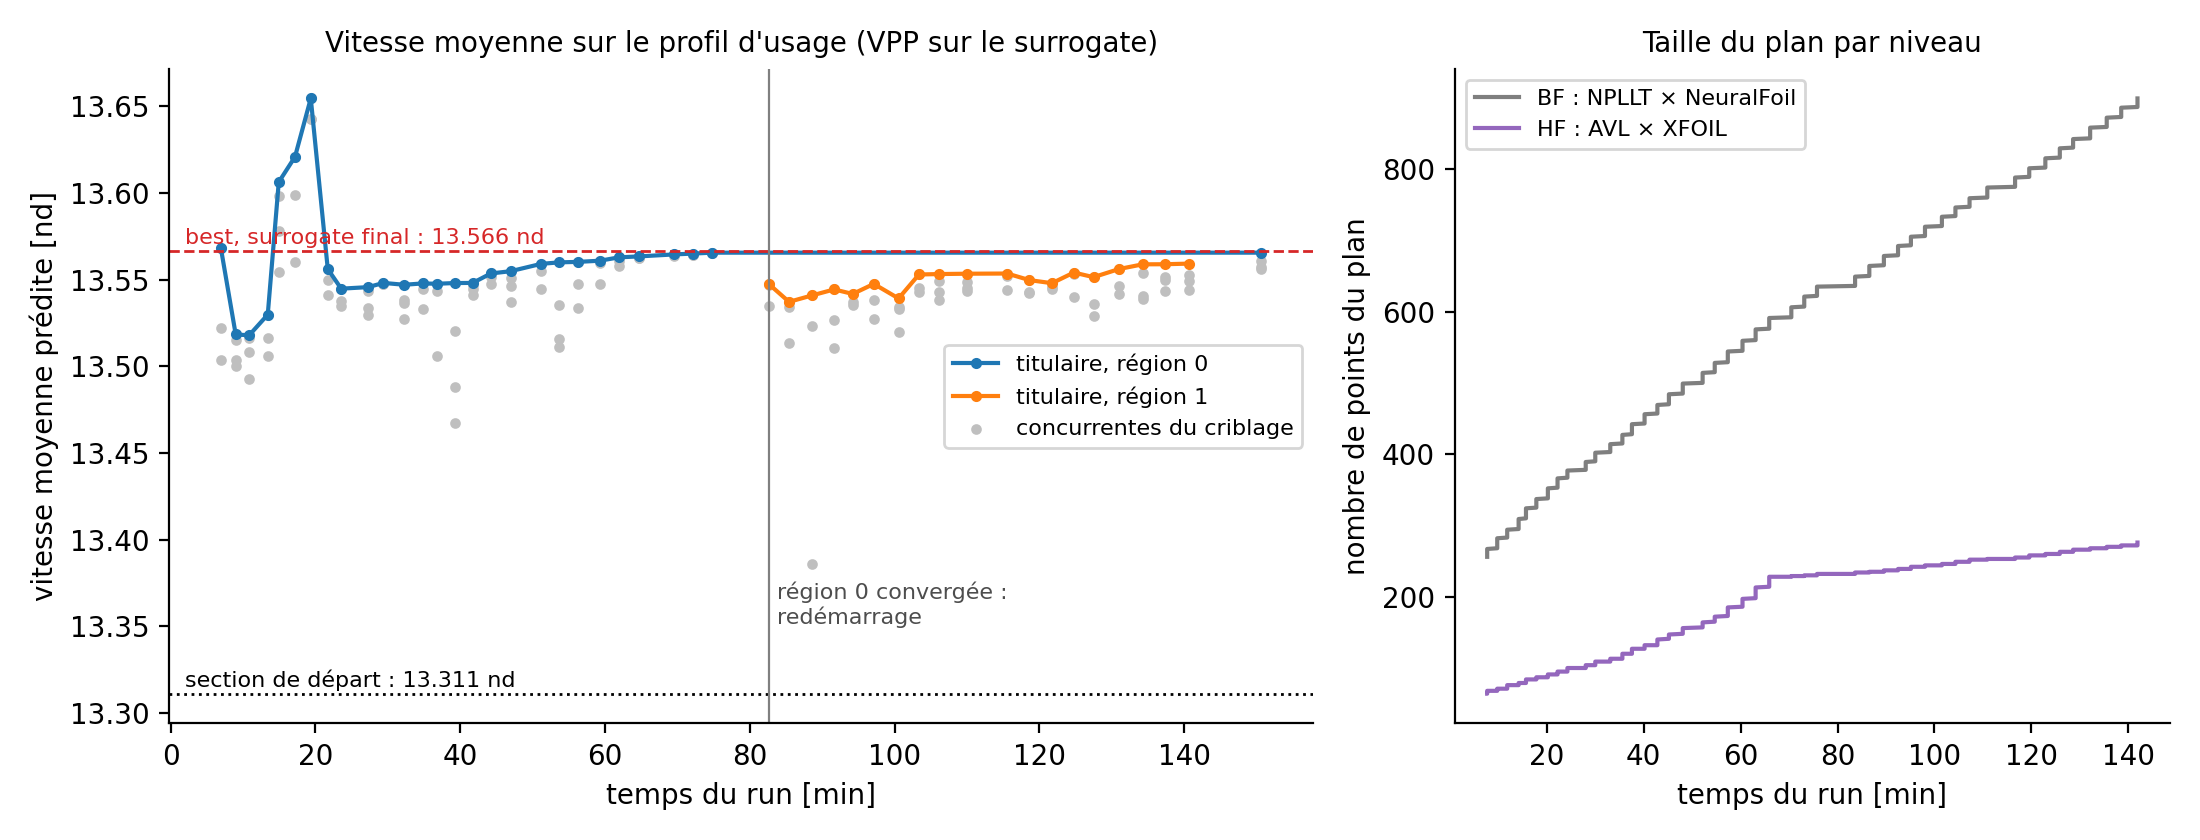
\includegraphics[width=\linewidth]{figures/run8_convergence.png}

\small
\raggedright
\begin{itemize}\setlength{\itemsep}{0pt}
  \item 0--20 min : modèle encore pauvre, vitesses optimistes (pic à 13,65 nd), corrigées dès que les calculs
        arrivent.
  \item 20--78 min : la région 0 monte lentement à 13,566 nd puis converge. Région 1 : un autre bassin, plafonné à
        13,560 nd. C'est un plateau.
  \item Plan final : 899 points BF, 276 HF. Les HF se concentrent dans la première heure.
\end{itemize}
\end{frame}

% ---------------------------------------------------------------------------------------------
\begin{frame}{Run 8 : les sections et le gain}
\centering
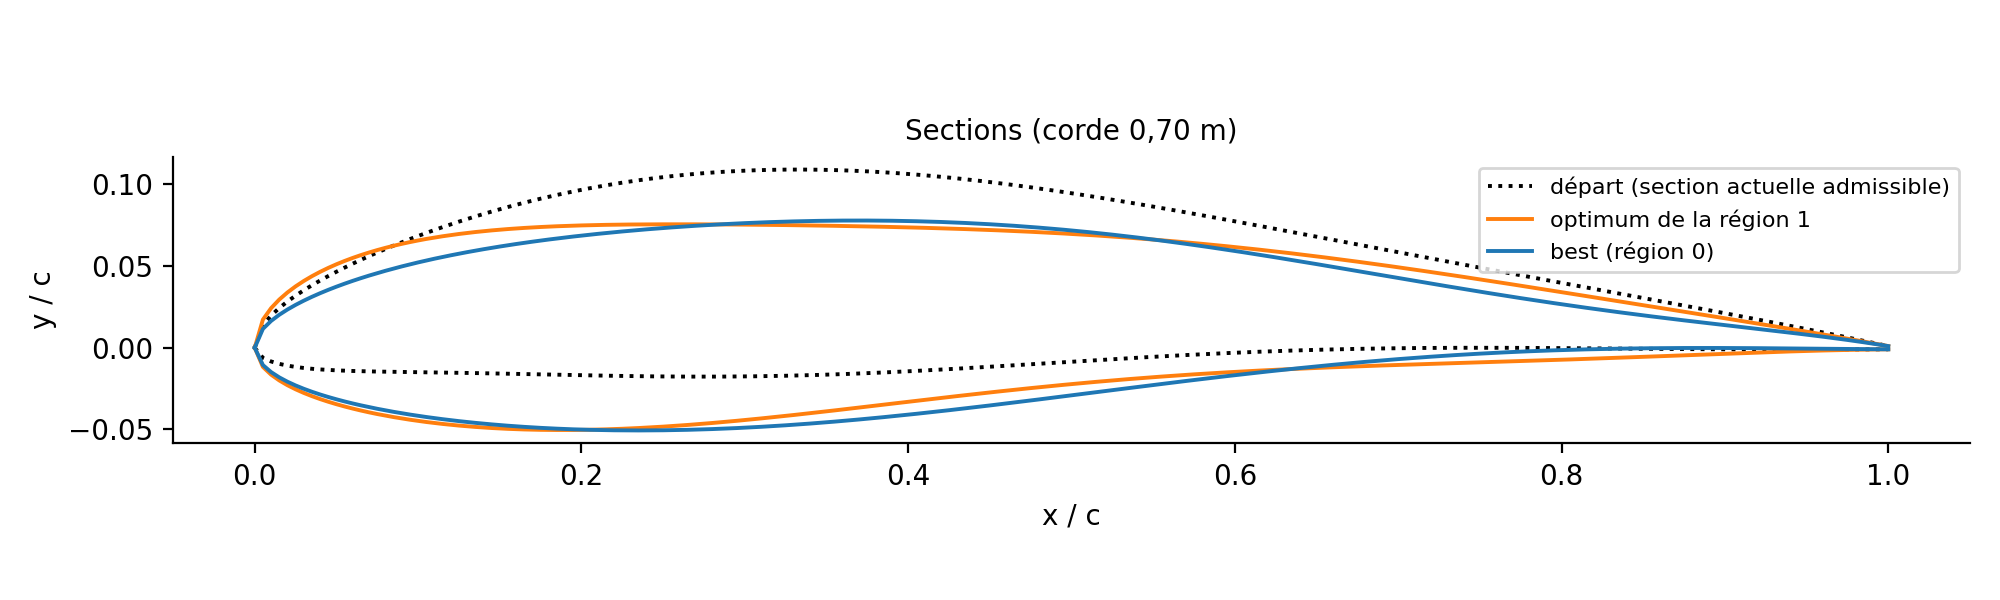
\includegraphics[width=0.78\linewidth]{figures/run8_sections.png}

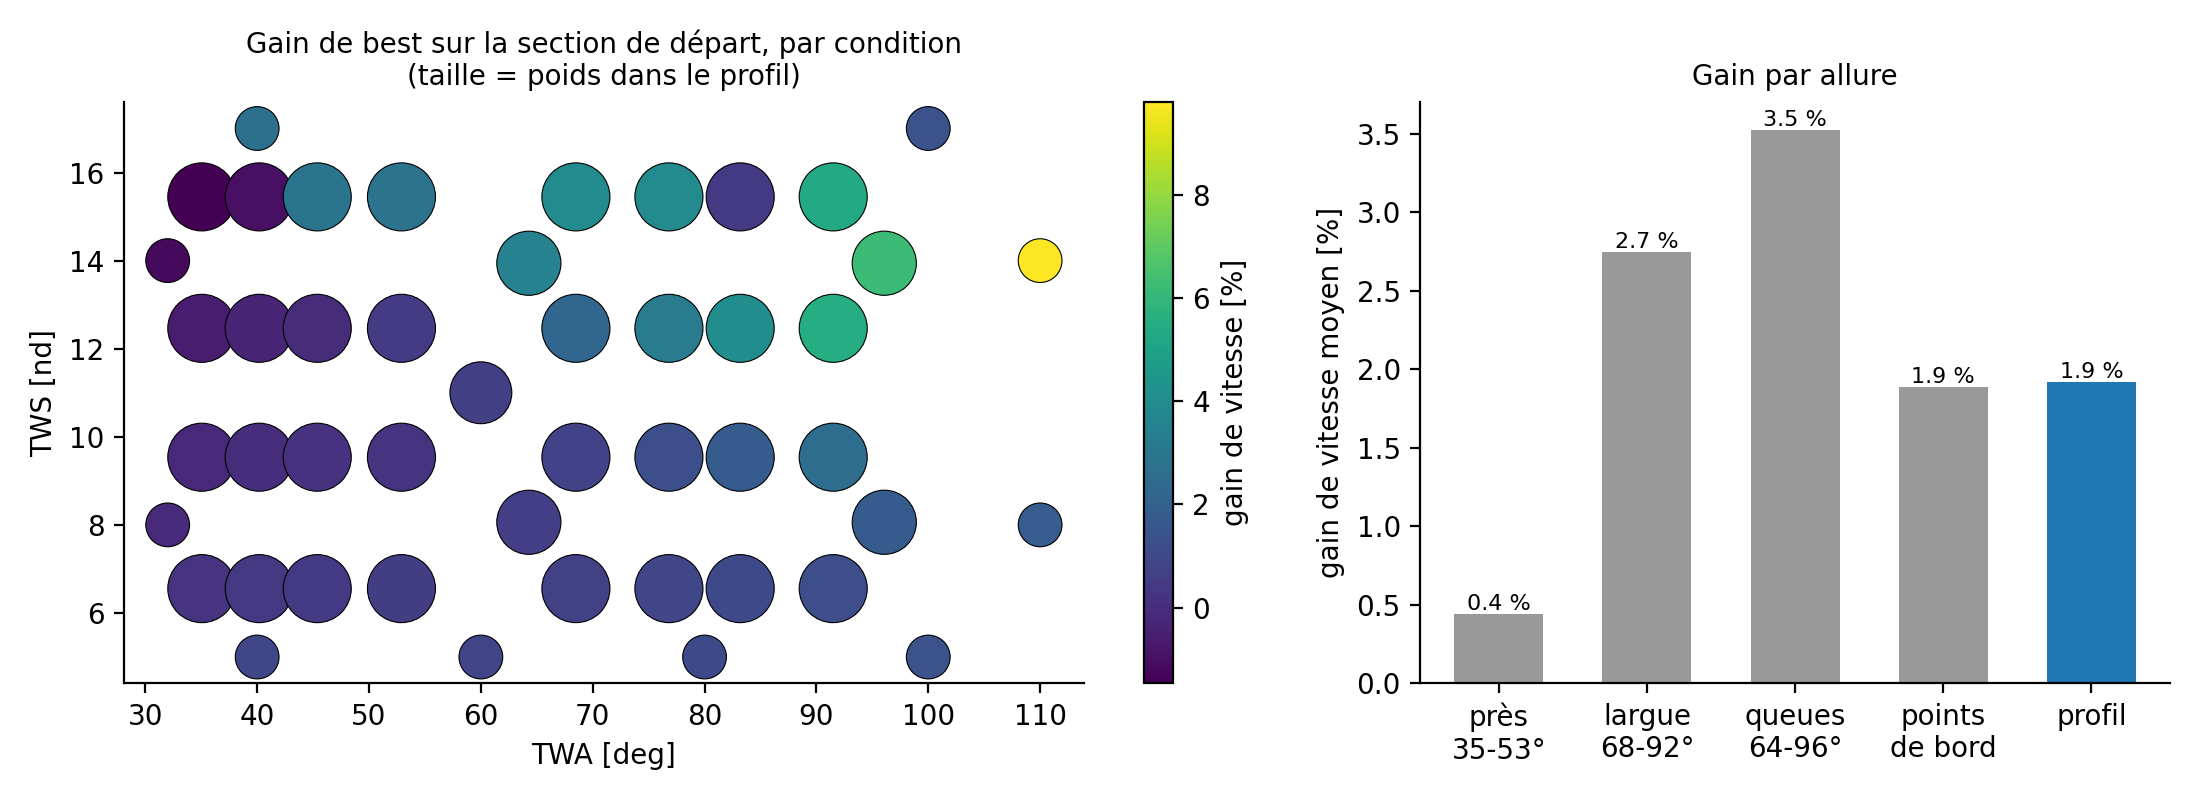
\includegraphics[width=0.78\linewidth]{figures/run8_gains.png}
\end{frame}

% ---------------------------------------------------------------------------------------------
\appendix
\begin{frame}{Réserve : le gain exact, tel que codé}
\small
Pour un candidat $(x, \ell)$, $\mathcal N_{ic}$ le nuage de $n$ points autour de l'état de la section $i$ à la
condition $c$ ($i$ = titulaire et 3 concurrentes) :
\[
  G(x, \ell) = \frac{1}{\mathrm{coût}(\ell)} \sum_{i} \sum_c \omega_c\,
  \frac1n \sum_{x' \in \mathcal N_{ic}} \sum_{k=1}^{6} d_{ck}^2\;
  r_k(x'; x, \ell)\tp\, \Lambda_k(x)^{-1}\, r_k(x'; x, \ell),
\]
\[
  r_k(x'; x, \ell) = \mathrm{Cov}\big(C_k^{\text{HF}}(x'),\, Y_{k}(x)\big),
  \qquad \Lambda_k(x) = \Var\big(Y_{k}(x)\big) + \text{bruit},
\]
$Y_k(x)$ le vecteur des observations nouvelles en $x$ : les niveaux manquants $\le \ell$ (plan emboîté), et
$\mathrm{coût}(\ell)$ leur coût cumulé.
\begin{itemize}\setlength{\itemsep}{2pt}
  \item Chaque terme $r\tp\Lambda^{-1}r$ est la baisse de variance de $C_k^{\text{HF}}(x')$ si l'on observe $Y_k(x)$ :
        la formule de conditionnement gaussien, avec les covariances entre niveaux du co-krigeage.
  \item Poids d'un point du nuage : $\omega_c\, d_{ck}^2 / n$, avec $\sum_c \omega_c = 1$.
  \item Nuage : $\pm1^\circ$ (cant), $\pm0{,}3^\circ$ (rake), $\pm1^\circ$ (yaw) ; avec la recherche locale, la moitié
        des points déplace aussi la section du rayon de la région de confiance.
  \item C'est une IMSE pondérée (Le Gratiet \& Cannamela 2015), avec une mesure d'intégration concentrée près des
        états de la VPP.
\end{itemize}
\end{frame}

\end{document}
